\documentclass[border=10]{standalone}
\usepackage{tikz}
\usepackage{pgfplots}

\tikzset{declare function={inverf(\x)=\x/abs(\x) * sqrt( sqrt( (4.3307 + ln(1-\x^2)/2 )^2 - ln(1-\x^2)/0.147 ) - (4.3307 + ln(1-\x^2)/2));}}
\tikzset{declare function={quantile(\x)=1.4142136 * inverf(2*\x - 1);}}
\tikzset{declare function={chauvenet(\x)=abs(quantile(1/(4*\x)));}}

\begin{document}
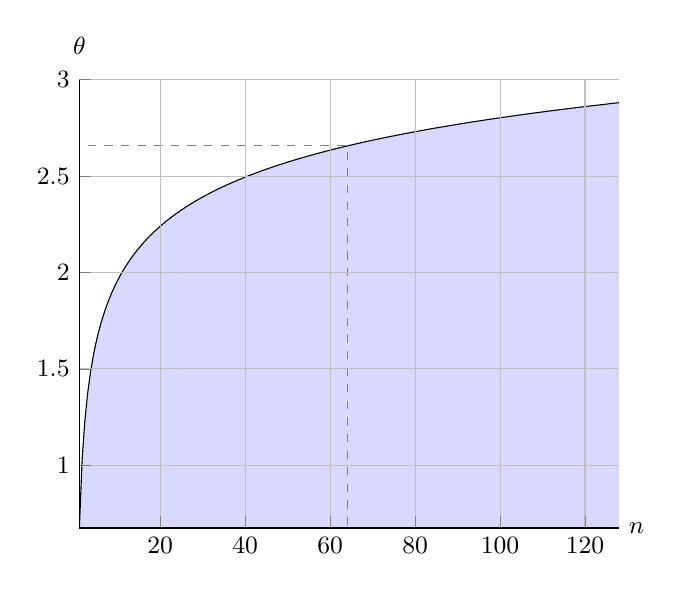
\begin{tikzpicture}[
  scale=1.0,
  every node/.append style={transform shape},
  font=\small
  ]
\begin{axis}[
  no markers,
  samples=200,
  domain=1:128,
  ymax=3,
  axis lines*=left,
  every axis x label/.style={at={(current axis.right of origin)},anchor=west},
  every axis y label/.style={at={(current axis.north west)},above=2mm},
  xlabel={$n$},
  ylabel={$\theta$},
  grid=major,
  axis on top,
  enlargelimits=false
  ]
  \addplot [draw=none,fill=blue!15!white] {chauvenet(x)} -- (128,0);
  \addplot [draw=black] {chauvenet(x)};
  \draw [draw=gray,dashed] (axis cs:64,0) -- (axis cs:64,2.66) -- (axis cs:0,2.66);
\end{axis}
\end{tikzpicture}
\end{document}
